\documentclass{beamer}
\usepackage[latin1]{inputenc}
\usepackage{xcolor}
\usepackage{hyperref}
\usepackage{minted}
\usepackage{graphicx}
\usepackage{siunitx}
\usepackage{tikz}
\usetikzlibrary{shapes,fit,positioning,calc}
\usepackage{bbding} % For \HandRight
\usepackage{fancyvrb} % For \UseVerb \SaveVerb

\usetheme{Madrid}
\usecolortheme{default}

% Command that embeds a hand pointing to the right in a href label
\newcommand{\hrefhand}[2]{\raisebox{-0.4ex}{\HandRight}\,\href{#1}{#2}}

\title{COMP3320 Introduction to OpenGL}
\author{Alex Biddulph}
\institute{
    The University of Newcastle, Australia
    \and
    Based on the work provided at \url{www.learnopengl.com}
}
\date{Semester 2, 2021}

\begin{document}

\begin{frame}
    \titlepage
\end{frame}

\begin{frame}[fragile]{Blinn-Phong Lighting}
    \begin{itemize}
        \item Specular lighting breaks down when the angle between the view and light direction vectors exceeds \ang{90}
        \item Harsh cutoff appears when the angle exceeds \ang{90}
    \end{itemize}

    \begin{figure}
        \centering
        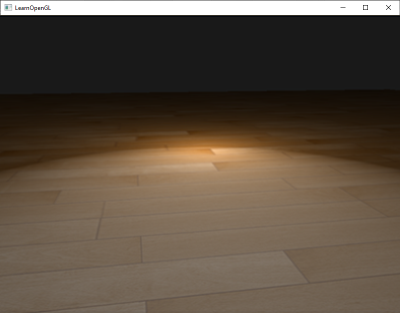
\includegraphics[height=0.50\textheight]{images/advanced_lighting_phong_limit.png}
        \caption{\footnotesize{Image sourced from \url{learnopengl.com/Advanced-Lighting/Advanced-Lighting}}}
    \end{figure}
\end{frame}

\begin{frame}[fragile]{Blinn-Phong Lighting}
    \begin{itemize}
        \item Rather than using the reflected vector use the halfway vector, the vector exactly halfway between the view and lighting directions $$\vec{H} = \frac{\vec{L} + \vec{V}}{\|\vec{L} + \vec{V}\|}$$
        \item Specular calculation then reduces to
              \footnotesize{
                  \begin{minted}{glsl}
vec3  norm        = normalize(frag_normal);
vec3  light_dir   = normalize(frag_pos - light_pos);
vec3  view_dir    = normalize(view_pos - frag_pos);
vec3  halfway     = normalize(view_dir + light_dir);
float strength    = pow(max(dot(norm, halfway), 0.0f), 32.0f);
vec3  specular    = 0.5f * strength * light_colour;
vec3  result      = specular * object_colour;
\end{minted}
              }
    \end{itemize}
\end{frame}

\begin{frame}[fragile]{Normal Mapping}
    \begin{itemize}
        \item We are modelling ``bumpy'' surfaces with flat triangles
        \item Vertex normals are useful for creating some nice lighting effects, but are not fine-grained enough to
              show shadows from bumps in the objects surface
        \item Textures fail to show the more detailed bumps in the object though
    \end{itemize}

    \begin{figure}
        \centering
        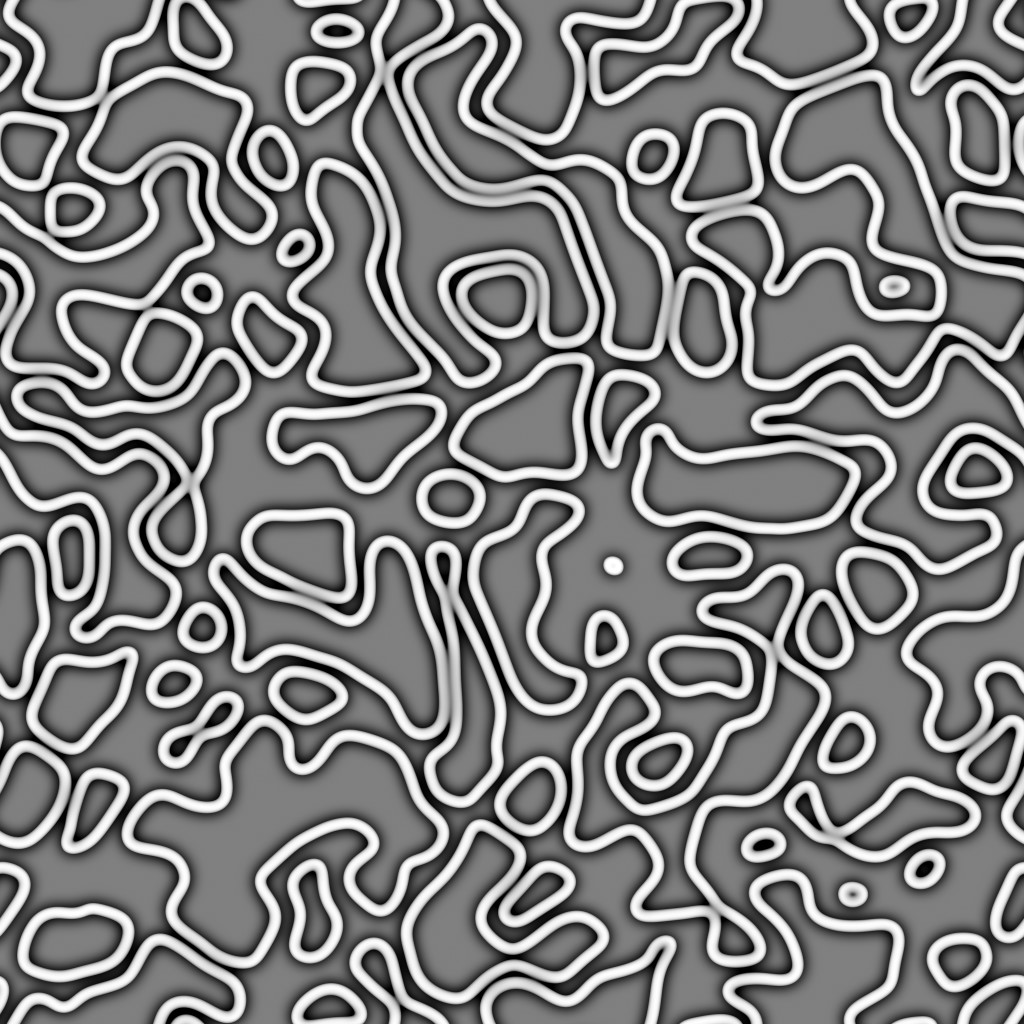
\includegraphics[height=0.50\textheight]{images/Abstract_005_COLOR.jpg}
        \caption{\footnotesize{Image sourced from \url{https://3dtextures.me/2017/12/28/abstract-005/}}}
    \end{figure}
\end{frame}

\begin{frame}[fragile]{Normal Mapping}
    \begin{itemize}
        \item Bake normal vectors into a texture, a ``normal map''
        \item Sample normal map to get normal vector for the current fragment
        \item Use this normal for lighting equations
    \end{itemize}

    \begin{figure}
        \centering
        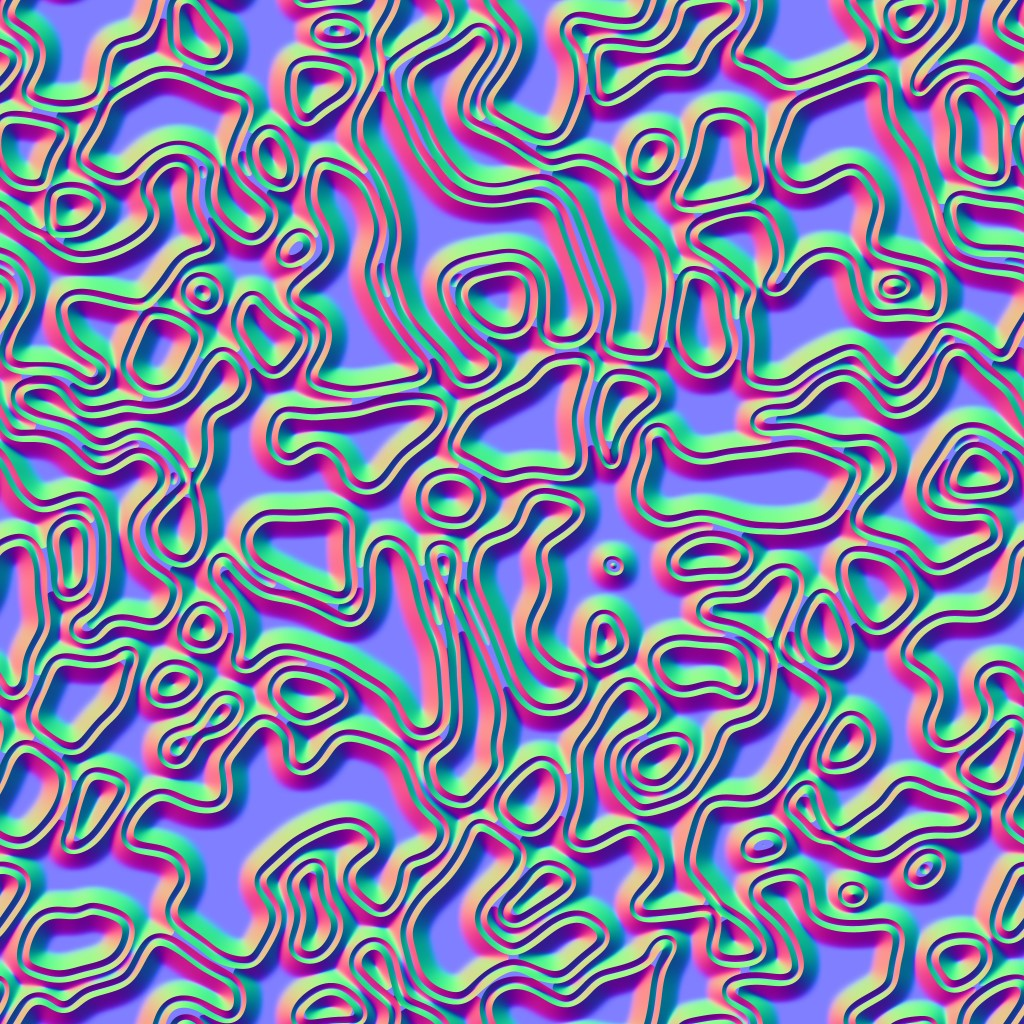
\includegraphics[height=0.50\textheight]{images/Abstract_005_NORM.jpg}
        \caption{\footnotesize{Image sourced from \url{https://3dtextures.me/2017/12/28/abstract-005/}}}
    \end{figure}
\end{frame}

\begin{frame}[fragile]{Normal Mapping}
    \begin{itemize}
        \item Creating the texture maps the normals to the range $\left[0, 255\right]$
        \item Texture sampling maps the normals to the range $\left[0, 1\right]$
        \item Need to convert the samples back to the range $\left[-1, 1\right]$
              \footnotesize{
                  \begin{minted}{glsl}
vec3 normal = vec3(texture(normal_map, texCoords));
normal      = normalize(normal * 2.0 - 1.0);
\end{minted}
              }
    \end{itemize}
\end{frame}

\begin{frame}[fragile]{Normal Mapping}
    \begin{figure}
        \centering
        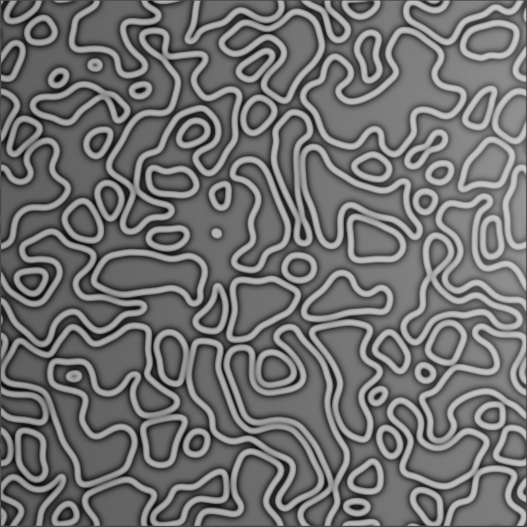
\includegraphics[height=0.50\textheight]{images/diffuse_only.png}
        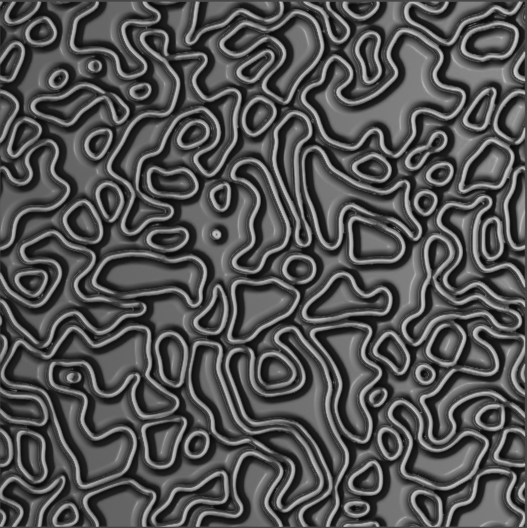
\includegraphics[height=0.50\textheight]{images/diffuse_with_normal.png}
        \caption{
            Left: Diffuse texture only. Right: Diffuse texture with normal map.
            \footnotesize{Image sourced from \url{https://3dtextures.me/2017/12/28/abstract-005/}}}
    \end{figure}
\end{frame}

\begin{frame}[fragile]{Tangent Space}
    \begin{itemize}
        \item Normal vectors in normal maps are expressed in tangent space
        \item Tangent space normals always point in the positive z direction (roughly)
        \item Need to account for this in lighting calculations
        \item Two options
              \begin{enumerate}
                  \item Map normal vectors from tangent space to world space
                  \item Map light positions from world space to tangent space
              \end{enumerate}
        \item Option one needs to happen in the fragment shader (happens once per fragment)
        \item Option two can be done in the vertex shader (happens once per vertex)
        \item There are typically a lot less vertices than there are fragments
    \end{itemize}
\end{frame}

\begin{frame}[fragile]{Tangent Space}
    \begin{itemize}
        \item The $TBN$ matrix will transform vectors from tangent space to world space
        \item The inverse of this matrix will transform world space vectors to tangent space
        \item $TBN = \left[\textrm{Tangent}|\textrm{Bitanget}|\textrm{Normal}\right]$
        \item Tangent, bitanget, and normal vectors need to be calculated per-vertex
        \item Can calculate all of these manually, or you can ask assimp to do it for you
    \end{itemize}
    \begin{examples}
        See \hrefhand{https://learnopengl.com/Advanced-Lighting/Normal-Mapping}{\color{blue}learnopengl.com} for a more detailed explanation of tangent space and the tangent and bitangent vectors
    \end{examples}
\end{frame}

\begin{frame}[fragile]{Tangent Space}
    \begin{itemize}
        \item Provide tangent, bitangent, and normal vectors to your vertex shader as uniforms
        \item These vectors will be in model space, need to convert them to world space
              \footnotesize{
                  \begin{minted}{glsl}
vec3 T = normalize(vec3(Hwm * vec4(aTangent, 0.0)));
vec3 B = normalize(vec3(Hwm * vec4(aBitangent, 0.0)));
vec3 N = normalize(vec3(Hwm * vec4(aNormal, 0.0)));
mat3 TBN = mat3(T, B, N);
\end{minted}
              }
        \item Strictly speaking you don't need to provide the bitangent vector
        \item $\vec{T}$, $\vec{B}$, and $\vec{N}$ are all orthogonal to each other, so given $\vec{T}$ and $\vec{N}$ we can calculate $\vec{B}$ as $$\vec{B} = cross\left(\vec{N}, \vec{T}\right)$$
    \end{itemize}
\end{frame}

\begin{frame}[fragile]{Tangent Space}
    \begin{itemize}
        \item With complex models with lots of vertices being shared between triangles it is possible to end up with $\vec{T}$, $\vec{B}$, and $\vec{N}$ not being mutually orthogonal
        \item If you think this is causing your normal mapping to be slightly off the Gram-Schmidt process can be used to re-orthogonalise the vectors
              \footnotesize{
                  \begin{minted}{glsl}
vec3 T = normalize(vec3(Hwm * vec4(aTangent, 0.0)));
vec3 N = normalize(vec3(Hwm * vec4(aNormal, 0.0)));

// Ensure T is orthogonal to N
// If T is already orthogonal to N then
// dot(T, N) = 0, so T = T
T = normalize(T - dot(T, N) * N);

// Now calculate B to ensure all
// three vectors are mutually orthogonal
vec3 B = cross(N, T);

mat3 TBN = mat3(T, B, N);
\end{minted}
              }
    \end{itemize}
\end{frame}

\begin{frame}[fragile]{Displacement Mapping}
    \begin{itemize}
        \item Like normal mapping, displacement mapping is used to significantly increase the detail in our rendered objects
        \item Sample a texture and use the sampled value to shift the texture coordinates used for any other texture sampling
              \footnotesize{
                  \begin{minted}{glsl}
float height = texture(dispMap, texCoords);
vec2 p       = viewDir.xy / viewDir.z * (height * dispScale);
vec2 coords  = texCoords - p;

vec3 diffuse = texture(diffuseMap, coords);
vec3 normal  = texture(normalMap, coords);
normal       = normalize(normal * 2.0 - 1.0);
\end{minted}
              }
        \item $dispScale$ is an extra scaling factor to attenuate the effect of the displacement map
        \item Best to use a displacement map in conjuction with a normal map for best results
    \end{itemize}
\end{frame}

\begin{frame}[fragile]{Displacement Mapping}
    \begin{figure}
        \centering
        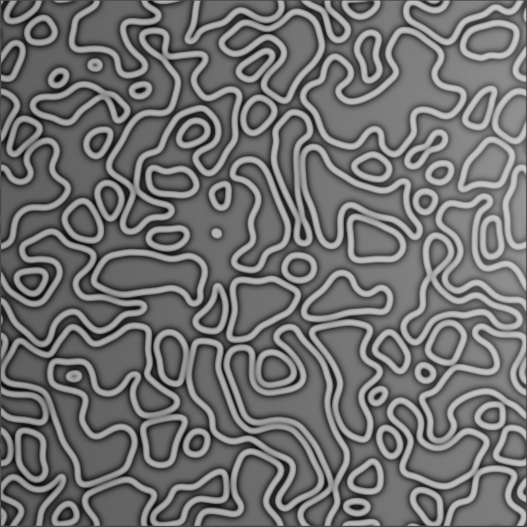
\includegraphics[width=0.30\linewidth]{images/diffuse_only.png}
        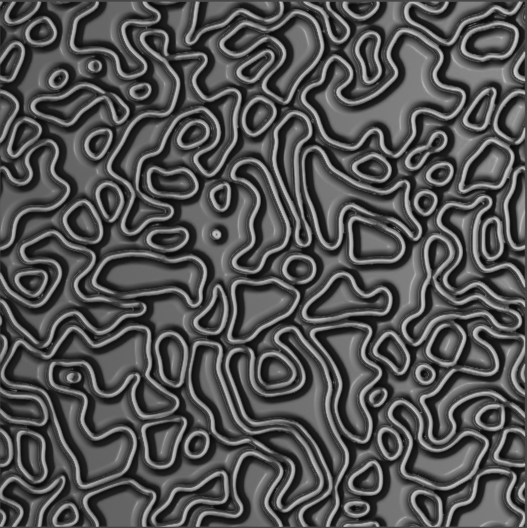
\includegraphics[width=0.30\linewidth]{images/diffuse_with_normal.png}
        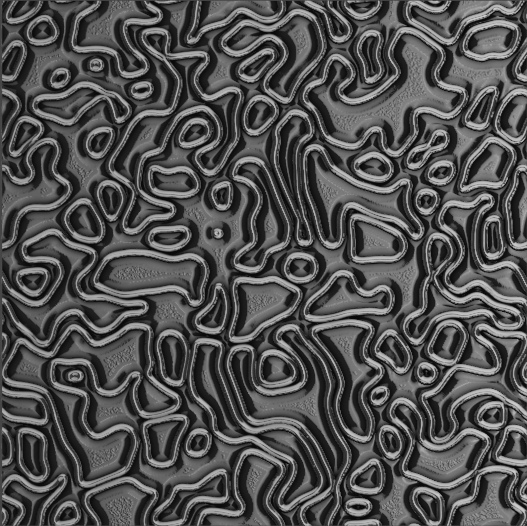
\includegraphics[width=0.30\linewidth]{images/diffuse_normal_displacement.png}
        \caption{
            Left: Diffuse texture only. Middle: Diffuse texture with normal map.
            Right: Diffuse texture with normal map and displacement map.
            \footnotesize{Image sourced from \url{https://3dtextures.me/2017/12/28/abstract-005/}}}
    \end{figure}
\end{frame}

\end{document}
